\section{Results Interpretation and Conclusions}
\label{sec:results}

\subsection{Key Findings}

One of the main findings we wanted to reveal is the UNSEEN MAP of New York. Figure \ref{fig:maxMapTotalPickDrop} shows the map. The colors of the map reveal the meaning of the yellow\_indicator. The NTAs in red correspond to those where the log scale of the number of pick ups was higher than a threshold (including UBER, Yellow cabs, Green cabs, and MTA entrance). The NTAs in yellow, correspond to those where the number of pick ups is zero or smaller than a threshold.

\begin{figure}%
\centering
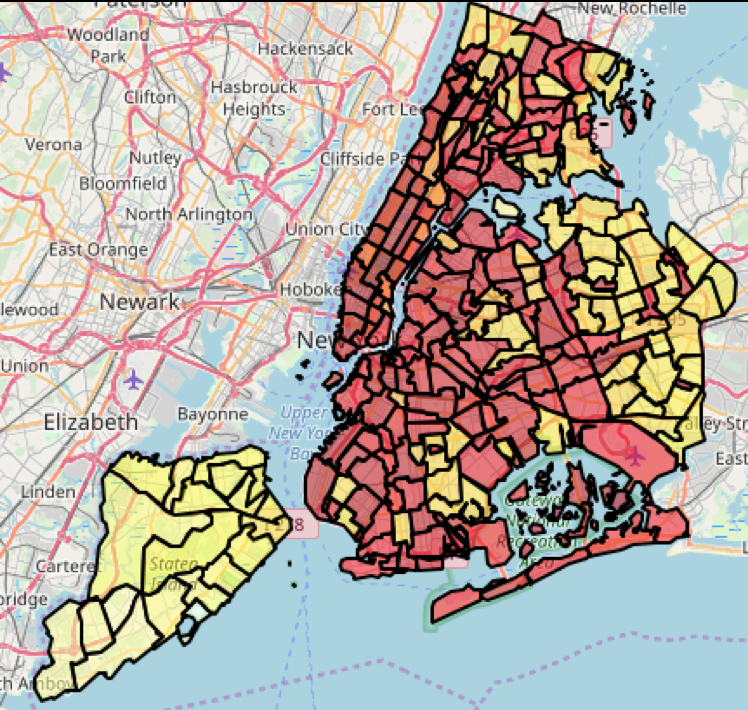
\includegraphics[height=5in, width=6.8in]{superMAP.png}
\caption{The UNSEEN Map of New York. The NTAs in red correspond to those where the log scale of the number of pick ups was higher than a threshold (including UBER, Yellow cabs, Green cabs, and MTA entrance)}
\label{fig:maxMapTotalPickDrop}%
\end{figure}


The maps reveal:

\begin{itemize}
\item  Possible areas unattended by different transportation means (yellow areas).
\item  An idea of people's mobility choices, depending on where they live. Red areas correspond to the ones that frequently use public transportation. Yellow areas correspond to the ones that use other options, either because they want or because they do not have other options.
\end{itemize}


From the Exploratory Data Analysis that was conducted and some statistical analysis we can conclude that:

\begin{itemize}
\item New York City has a lot to do in terms of mobility, especially for people that live in the outer NTAs. 
\item  People that live in the yellow areas have good incomes. So we could conclude that they use other transportation means such as their own car for long distance trips, or bikes, scooters, or even walk for short distances
\item Uber is one of the services that is attending the outer NTAs. However, not with a very high demand yet. 
\item The average distance of Green cabs have reduced from 2014 to 2015.  
\item The number of Uber trips are increasing and it looks to affect the number o trips made by Yellow and Green cabs.

\end{itemize}

All the notebooks with the code used to generate this report can be found in the following 
\href{https://github.com/jssalamanca1967/ds4a_datathon_group03}{Link}

Finally, to accomplish what was shown in this document, the work was divided as follows:

\begin{itemize}

\item Database AWS Computation / SQL queries: Alvaro Mu\~noz and Mario Cer\'on
\item Front End Dash App: Javier Coconubo, Jhonatan Salamanca and Jairo Ni\~no
\item Data Wrangling: Javier Coconubo, Carol Martinez, Jhonatan Salamanca and Alvaro Mu\~noz.
\item Dataset Research: Jairo Ni\~no and Carol Martinez
\item Project Management: Mario Cer\'on and Javier Coconubo
\item Documentation and reporting: Carol Martinez and Mario Cer\'on

\end{itemize}

All of the 6 members of the group collaborate in equal efforts as well. ($16,6\%$) 
